\documentclass[a4paper,14pt]{beamer}


\usetheme[progressbar=frametitle]{metropolis}
\usepackage{appendixnumberbeamer}
\usefonttheme{serif}
\usepackage{booktabs}
\usepackage[scale=2]{ccicons}

\usepackage{pgfplots}
\usepgfplotslibrary{dateplot}

\usepackage{xspace}
\newcommand{\themename}{\textbf{\textsc{metropolis}}\xspace}



\usepackage[slovene]{babel}
\usepackage[utf8]{inputenc}
\usepackage[T1]{fontenc}
\usepackage{amsmath}  % razna okolja za poravnane enačbe ipd.
\usepackage{amsthm}   % definicije okolij za izreke, definicije, ...
\usepackage{amssymb}  % dodatni matematični simboli
\usepackage{xypic}
\usepackage{relsize}
\usepackage{pgfpages}
\usepackage{tikz}
\usetikzlibrary{automata, positioning}

\beamertemplatenavigationsymbolsempty


%\beamerdefaultoverlayspecification{<+ ->}
\def\N{\mathbb{N}} % mnozica naravnih stevil
\def\Z{\mathbb{Z}} % mnozica celih stevil
\def\Q{\mathbb{Q}} % mnozica racionalnih stevil
\def\R{\mathbb{R}} % mnozica realnih stevil
\def\C{\mathbb{C}} % mnozica kompleksnih stevil
\newcommand{\geslo}[2]{\noindent\textbf{#1} \quad \hangindent=1cm #2\\[-1pc]}
\DeclareMathOperator{\diam}{diam}
\DeclareMathOperator{\Cay}{Cay}
\DeclareMathOperator{\Stab}{Stab}


\def\qed{$\hfill\Box$}   % konec dokaza
\def\qedm{\qquad\Box}   % konec dokaza v matematičnem načinu
\newtheorem{izrek}{Izrek}
\newtheorem{trditev}{Trditev}
\newtheorem{posledica}{Posledica}
\newtheorem{lema}{Lema}
\newtheorem{opomba}{Opomba}
\newtheorem{definicija}{Definicija}
\newtheorem{zgled}{Zgled}


% \usetheme{frankfurt}
% \usefonttheme{serif}
%\beamerdefaultoverlayspecification{<+ ->}

\title{Optimal search for rationals}
\author{Matej Cerar}
\date{21. 5. 2024}

\begin{document}


\maketitle


\begin{frame}
    \frametitle{Predstavitev problema}
    \begin{itemize}
        \item Kako optimalno poiskati racionalno število v seznamu oblike 
        $O_M = \{ p/q \text{ }| \text{ }p,q \in \{1,2, \cdots, M\}\}$, le z vprašanjem ali je izbrano 
        število manjše ali večje od x?
    \end{itemize}
    
\end{frame}


\begin{frame}
    \frametitle{Pregled reševanja}
    \begin{enumerate}
        \item Eksponentno iskanje intervala.
        \item Binarno iskanje celega dela.
        \item Isakanje dovolj majhnega ulomka.
        \item iskanje decimalnega dela.

    \end{enumerate}
    
\end{frame}


\begin{frame}
    \frametitle{Eksponentno iskanje celega dela}
        \begin{figure}
            \centering
            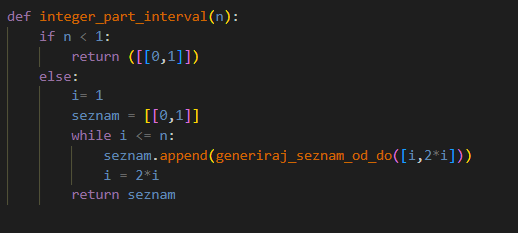
\includegraphics[width = 1\textwidth]{eksponentno.png}
            \caption{Coda za eksponentno iskanje}
        \end{figure}
\end{frame}

\begin{frame}
    \frametitle{Iskanje celega dela}
    \begin{columns}
        \begin{column}{0.5\textwidth}
         \begin{figure}
             \centering
             \includegraphics[width = 1.1\textwidth]{Iskanje_celega_dela_1.png}
             \caption{iskanje celega dela }
         \end{figure}
         
        \end{column}
        \begin{column}{0.5\textwidth}
         \begin{figure}
             \centering
             \includegraphics[width = 1.2\textwidth]{Iskanje_celega_dela_2.png}
             \caption{Iskanje celega dela }
         \end{figure}
         
        \end{column}
    \end{columns}
\end{frame}


\begin{frame}
    \frametitle{Lema 4 in iskanje intervala za decimalni del}
        \begin{figure}
            \centering
            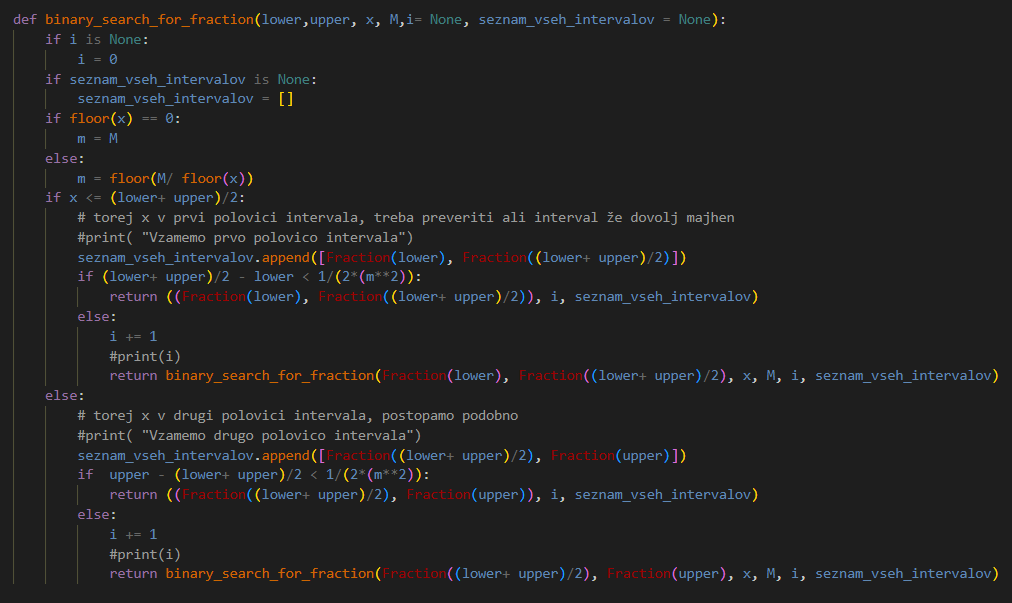
\includegraphics[width = 0.9\textwidth]{Iskanje_intervala_za_racionalni_del.png}
            \caption{Iskanje intervala za decimalni del}
        \end{figure}
\end{frame}



\begin{frame}
    \frametitle{Lema 5 in določitev iskane številke}
        \begin{figure}
            \centering
            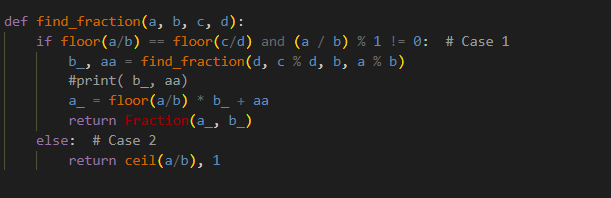
\includegraphics[width = 1\textwidth]{find_fraction.png}
            \caption{Iskanje izbrane številke}
        \end{figure}
\end{frame}

\begin{frame}
    \frametitle{Spletna stran}
       Implementacija spletne strani in predstavitev delovanja.
\end{frame}
\end{document}